\chapter{Documentation}
\begin{overview}
Two different types of documentation as well as the corresponding ISA identification numbering used by these documents are defined for used specifically in the process control laboratory. A formal representation of the experimental setups will greatly reduce the amount of time spent on fault debugging and control loop maintenance. The two documentation types used are:
\begin{description}
	\item[Piping and instrumentation diagrams] that are used to describe piping and equipment for the different \eindex{experimental setups}.
	\item[Loop diagrams] that are used to define the wiring of the different instrumentation loops.
\end{description} 
\end{overview}

\section{Piping and instrumentation diagrams}
A \eindex{piping and instrumentation diagram} (P\&ID) is a detailed graphic representation of the process flow showing all the piping, the equipment and much of the instrumentation associated with the given process \citep[93]{Mulley93}. The different equipment and instrumentation is identified using unique numbers called \eindex{tag numbers}. The \eindex{tag number} of the different instrumentation in the process control laboratory conforms to the \eindex{ISA standards} and are defined as follows:
\begin{center}
	\framebox{Unit number} \framebox{Identifier} \framebox{Loop number}
\end{center}

The different unit numbers specified can be seen in table~\ref{tab:wire:units} while the different identifiers needed to describe the current instrumentation in the process control laboratory is listed in table table~\ref{tab:wire:ident}. The loop number is a three digit number, and is unique to each measurement loop. The sensor, transmitter and controller will therefore have the same loop number with different identifiers.
\begin{table}[htbp]
	\centering
	\caption{Unit numbers of the process control laboratory}
\begin{tabular}{ll}
\toprule[1pt]
	Number & 	Setup name \\
\midrule[0.5pt]
	01 & Acetone flashing \\
	02 & pH \\
	03 & Temperature \\
	04 & Level and flow \\
	05 & Distillation \\
	06 & OPTO22 setup \\
\bottomrule[1pt]
	\end{tabular}
	\label{tab:wire:units}
\end{table}

\begin{table}[htbp]
	\centering
	\caption{Different object types}
	\begin{tabular}{l c | l c}
		\toprule[1pt]
			Instrument  &  Identifier & Instrument& Identifier \\
		\midrule[0.5pt]
		\emph{Sensors}							 &        &                            &    \\
			Thermocouple    					 & TE     & \emph{Other} \\
			RTD					    					 & TE 		& Analog temperature controller & TC \\
			Differential pressure cell & DP 		& E/P converter							 & PY \\
			pH probe			  					 & XE 		&	Power supply               & ES \\
			Flow sensor								 & FE 		& \eindex{Junction box}      & TB \\
			Level sensor							 & LE     & \eindex{Opto box rail}     & TS \\ 
																 &        & \eindex{SNAP module}			 & OP \\													
		\emph{Transmitters} 				 &				& 													 &    \\
			Wheatstone bridge					 & TT 		& \emph{Vessels}\\
			pH transmitter						 & XT 		& Tank											 & TK \\
			Level transmitter					 & LT 		& Pump											 & CP \\
			Flow transmitter 					 & FT 	  & Heat exchanger						 & HE \\
								 								 &				& Hand valve								 & HV \\	
		\emph{Actuators}						 &				& Vapour liquid equilibrium  & VL \\
			Thyristor									 & VC \\		
			Control valve							 & CV \\
		\bottomrule[1pt]
	\end{tabular}
	\label{tab:wire:ident}
\end{table}

A list of the different symbols used in the representation of processing equipment is available in the following two references \emph{Chemical Engineering Drawing Symbols} or \emph{Control System Documentation, Applying Symbols and Identifications}. 

\begin{example}
	The tag numbering, defined from table~\ref{tab:wire:ident}, of the instrumentation and processing equipment used for a simplified pH control loop is listed in table~\ref{tab:docu:examp}.
	\begin{table}[htbp]
		\centering
		\caption{Tag number identification}
			\begin{tabular}{l l}
			\toprule[1pt]
				Instrument type & Tag number \\
			\midrule[0.5pt]
				pH sensor			  & 02XI001 \\
				pH transmitter  & 02XT001 \\
				Analog input channel & 06OP235\\
				Control valve   & 02CV001 \\
				I/P converter   & 02PY001 \\
				Analog output channel & 06OP208\\
				Tank            & 02TK001 \\
			\bottomrule[1pt]
		\end{tabular}
		\label{tab:docu:examp}
	\end{table}
	
	The P\&ID for the pH control system can accordingly be drawn using the different tag numbers of the 								instrumentation as well as the standard symbols for vessels and instrumentation. The resulting P\&ID can be seen 		in figure \ref{fig:docu:examp}. 
	\begin{figure}[htbp]
		\centering
		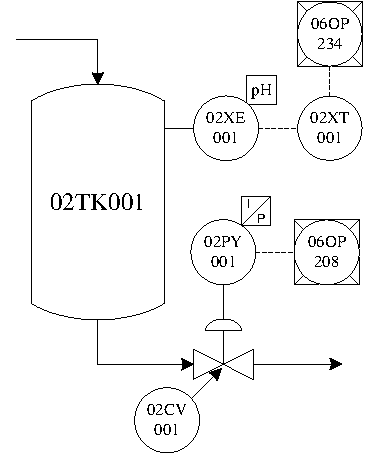
\includegraphics[width = 0.45\textwidth]{docupid}
		\caption{Cable marking}
		\label{fig:docu:examp}
	\end{figure}

	The I/P converter and pH sensor have individual identification blocks denoting the conversion and measurement of 		the different instrumentation.
\end{example}

\section{Loop diagrams}
The wiring system has many connections that must be documented in an efficient unambiguous way. The standard format used for the documentation of analog and digital control loops are \eindex{loop diagrams}\citep[143]{Mulley93}. An example of the loop diagram for the two control valves of the pH control loop in the control laboratory can be seen in figure~\ref{fig:wire:wired}.
\begin{sidewaysfigure}[p]
	\centering
	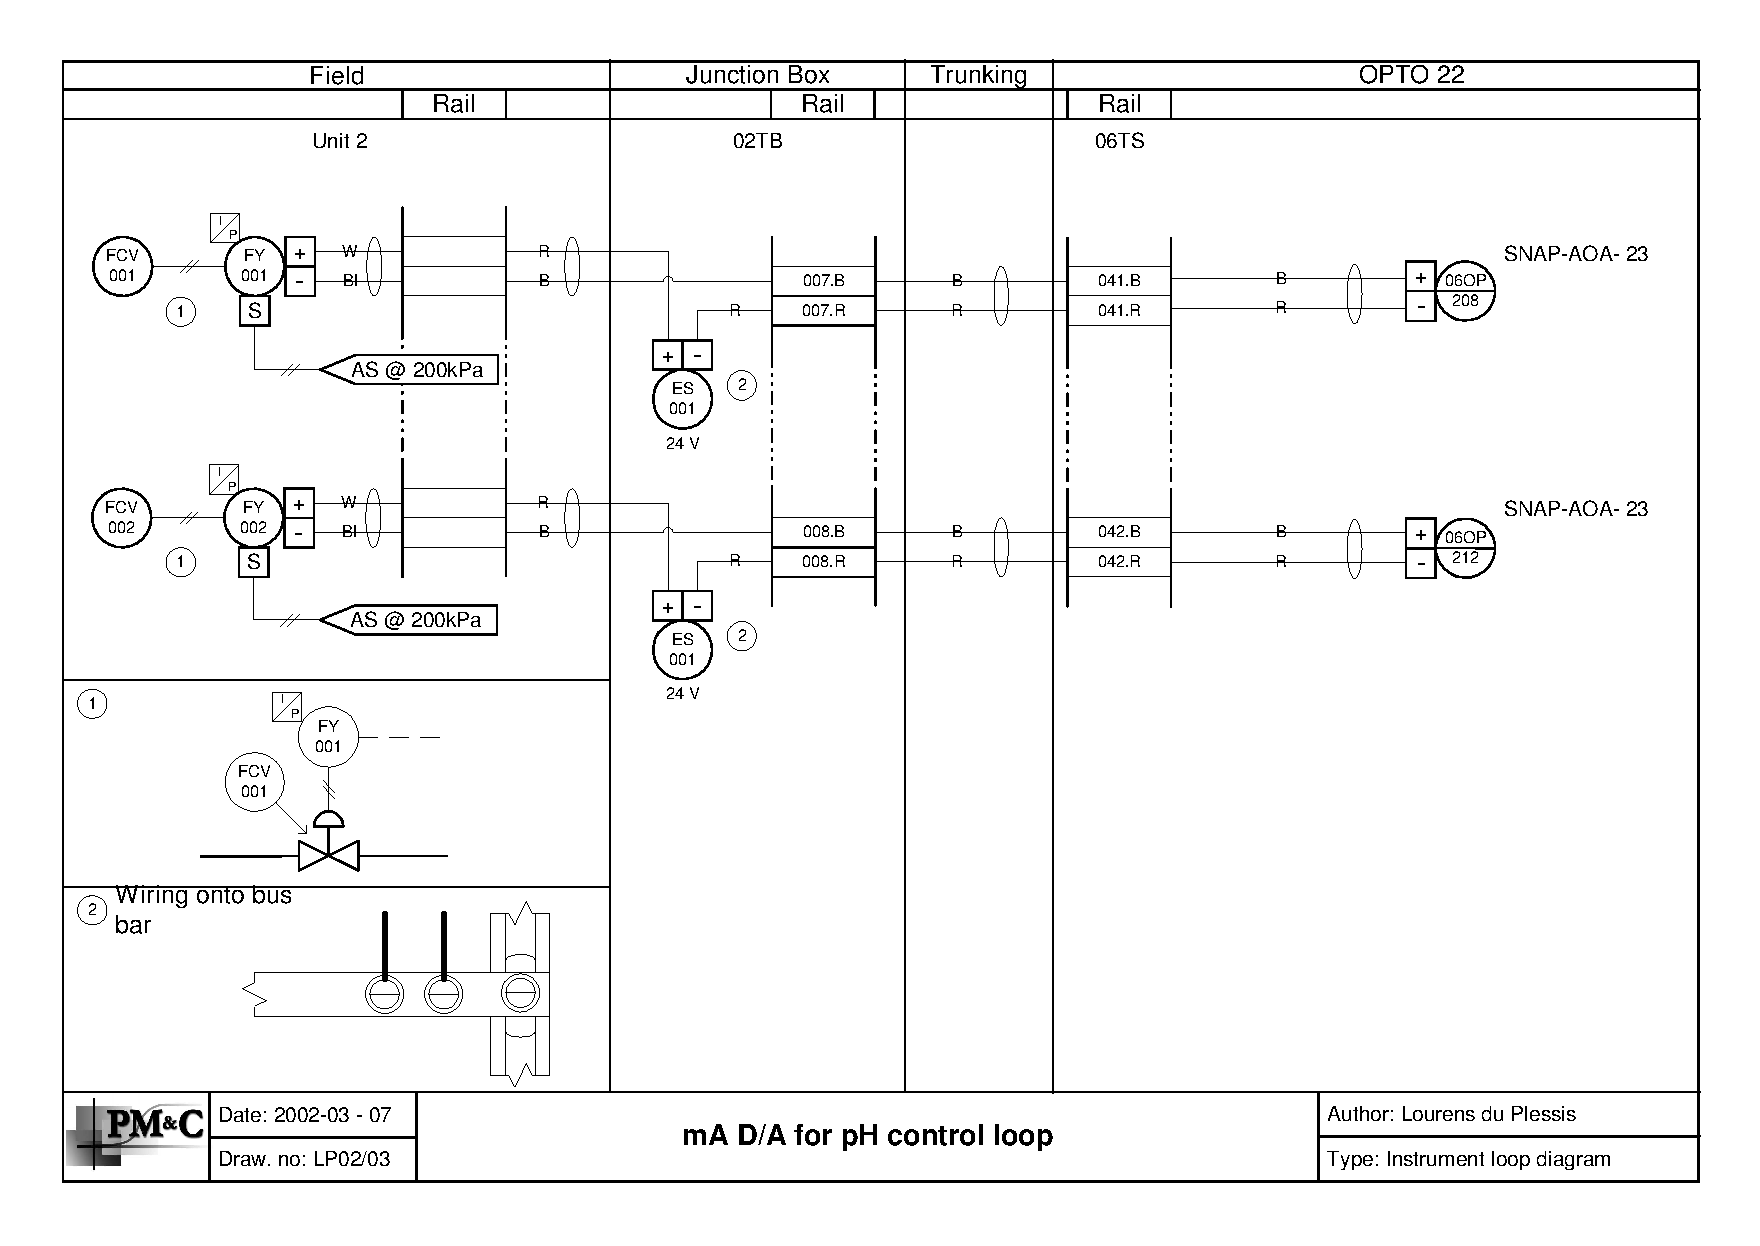
\includegraphics[width = \textwidth]{wirewired}
	\caption{Wire diagram of the control valves of the pH control loop}
	\label{fig:wire:wired}
\end{sidewaysfigure}

It can be seen that the electrical wiring of the system is shown with the associated instrumentation of the loop. The diagram will therefore greatly assist in the detection and correction of faults or the installation of new instrumentation. The diagram consist further out of four main areas, separated by vertical lines the definition of these areas follows.
\begin{description}
	\item[Field] defines the instrumentation on the experimental setup. The instrumentation usually associated with the field are are sensors, actuators, converters and transmitters.
	\item[Junction box] defines the wiring inside the junction box. The power supply and connectors with their corresponding identification number or tag are clearly shown. It should be noted however that the full connector number consist out of the number shown on the connector as well as the rail number. The tag number for the connector is therefore 02TBXXX.C with the C denoting either the red (R) or blue (B) wire.
	\item[Trunking] is the wiring between the \eindex{junction box} and the \eindex{Opto box}.
	\item[OPTO22] is the instrumentation inside the \eindex{Opto box}. The connectors are again shown with the \eindex{SNAP modules}. The Opto box is allocated unit number six 06, the connector tag number will therefore be 06TSXXX.C. The two opto racks are defined by numbers 1 and 2. The tag number for a specific measurement will therefore be 06OP1XX or 06OP2XX depending on the associated rack of the current model.  
\end{description}

\section{Tag number marking}
\subsection{Cable marking}
The numbering of the different cables are affixed to the cable using specific colour coded cable markers. The cable number contains two parts, the connector number from the cable origin and the connector number of the destination connector. 

The cable number is affixed on both ends of the cable. The exact source and  origin of the cable can accordingly be seen at any end; reducing the effort for maintenance and fault detection. The connectors are marked as well using smaller plastic numbering clips with the same colour scheme as that used for the cables. 

The direction of the numbering is always from the \eindex{experimental setup} to the \eindex{Opto box} with a dash separating the two numbers.  An example can be seen in figure~\ref{fig:wire:mark2} with the tag numbering flow from the experimental setup (001) to the Opto box (201), which is in this case from left to right.
\begin{figure}[htbp]
	\centering
	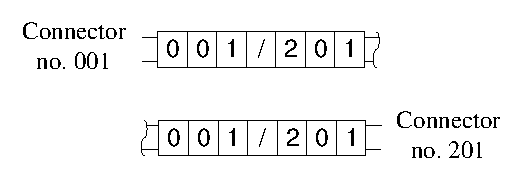
\includegraphics[width = 0.5\textwidth]{wiremark2}
	\caption{Cable marking}
	\label{fig:wire:mark2}
\end{figure}

\subsection{Instrument marking}
The instrumentation is marked clearly with a tag defining the full tag number of the instrument. ``Cable ties'' are used to fix the marker onto the instrumentation (see figure~\ref{fig:wire:valvemark}).
\begin{figure}[htbp]
	\centering
	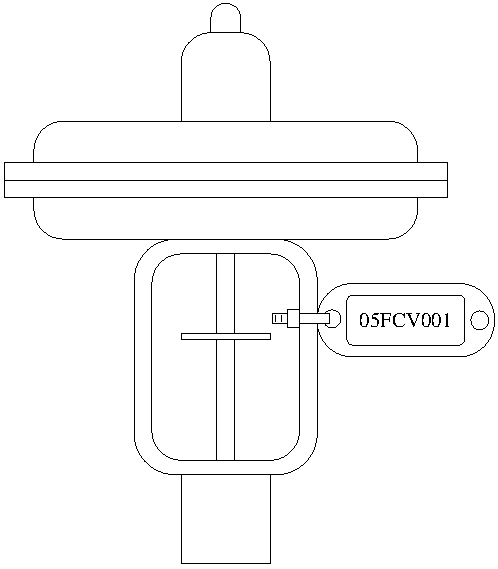
\includegraphics[width = 0.4\textwidth]{wirevalvemark}
	\caption{Instrument marking}
	\label{fig:wire:valvemark}
\end{figure}

\section{Equipment Database}
To simplify the documentation of the wiring and connectors, an \eindex{equipment database} is required. This database tracks each piece of process control equipment and the connections between them. The database can be obtained at $\backslash$$\backslash$groa$\backslash$phpMyAdmin.

The starting point for the database is the rig table, which contains the number and name of all the experimental setups.  From here, linked to the rig number an equipment table stores each item's type and number.  In addition, data is stored about the date of acquisition and origin of the equipment to simplify maintenance and reordering.  To make the database expendable, a table of equipment types is linked to the equipment table, storing the tag extension of the equipment type. 

Queries are defined to generate tag numbers in accordance with the standards set out above, by combining the rig number, equipment type extension and the equipment number.

In order to track connections, each equipment record also stores the unique ID of another piece of equipment.  The direction of this linked list is defined as away from the final control elements and measuring devices.  Therefore, a control valve will link to the \eindex{junction box} connector and an OPTO SNAP analog in module will link to the \eindex{junction box} connector.  

Wire names are generated by a \eindex{SQL query}, adding the numbers from the connected pieces of equipment.  A list of wire names can be drawn up in a report for wire checking. 

To keep the documentation current, the following steps are required when adding new equipment.
\begin{description}
\item[Step 1] Collect information
The following information is pertinent when installing new equipment:
\begin{itemize}
	\item	What type of signal does the equipment send or receive?  This will determine the module on the OPTO that the equipment will be wired to.
	\item	Are there enough connectors in the \emph{junction box} to accommodate the new signal?  If not, new connectors must be installed.
	\item	Are there enough OPTO modules of the type required? If not, a new OPTO module must be installed.
\end{itemize}

\item[Step 2] Add the equipment to the equipment database.
Check that the equipment type exist by double clicking the equipment type table.  If the equipment type does not exist, add a new type on the last line of the table and close the table view.  Open the equipment table by double clicking it.  Select the rig and equipment type from the drop down list.  Enter a unique number for the equipment in the number field, then select the tag number of the equipment this item is connected to.  For instance, a thermocouple would be connected to a connector in the \eindex{junction box} for the experimental setup. If there are no free connectors in the \eindex{junction box}, follow the same steps as above for two new connectors: one in the \eindex{junction box} and one in the \eindex{Opto box}.

\item[Step 3] Lay the wiring
Open the trunking and lay a new wire between the \emph{Opto box} and the \emph{junction box}, bearing in mind that the wire must be labelled with its wire number.  Use the wire number for the wire between the connectors mentioned above.  This number is generated automatically by the database in the wire numbers query.

\item[Step 4] Connect the wires
The wires are now connected between connectors.

\item[Step 5] Test
Before the equipment is used, a signal check must be run.  Using a Ohmmeter, check the resistance between the terminals of the new signal.  This should be very high.  Low values indicate a short circuit.

\item[Step 6] Connect equipment and OPTO
The wires are now connected to the equipment and to the OPTO module.
\end{description}

An example of the database interface can be seen in figure~\ref{fig:docu:interface} and shows the different experimental setups of the process control laboratory.
\begin{figure}[htbp]
	\centering
	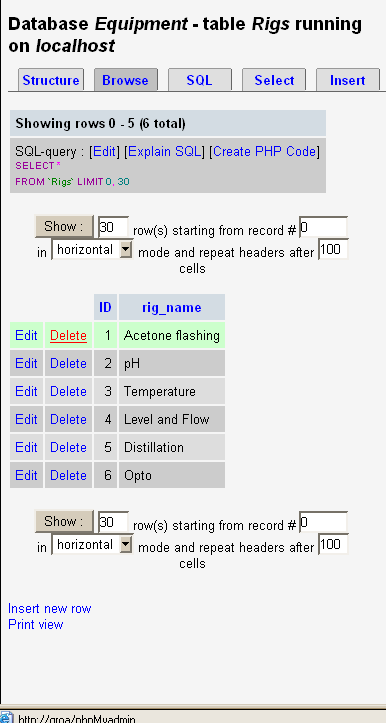
\includegraphics[width = 0.6\textwidth]{interface}
	\caption{Equipment database interface}
	\label{fig:docu:interface}
\end{figure}